\definecolor{exxetagray}{gray}{0.75}
\definecolor{itemcolor}{RGB}{179,217,255}
\definecolor{usercolor}{RGB}{255,204,179}

\shorthandoff{"}
\chapter{Empfehlungssysteme}
\label{ch:empfehlungssysteme}

\section{Einführung}
\label{ch:empfehlungssysteme:einfuehrung}
\textcite[S. 1ff.]{malinowski:2006} zu Folge sollte das Konzept des \acp{PEFit} auch bei der automatisierten Personalauswahl bzw. Stellensuche Berücksichtigung finden. Bei solchen Problemstellungen eingesetzte Computeranwendungen werden als Empfehlungssysteme bezeichnet. Sie verfolgen das Ziel, für eine große Menge von Elementen vorherzusagen, wie gut diese für ein Anliegen eines Nutzers geeignet sind und sie in der entsprechenden Reihenfolge zu sortieren \cite[S. 3]{recommenderSystems:2016}. Häufig entfällt dabei für den Anwender vollständig die Notwendigkeit einer manuellen Suche \cite[S. 1]{comibingCareer:2013}. 

Im englischsprachigen Raum ist der Begriff des Empfehlungssystems auch unter Bezeichnungen wie Recommender System \cite[S. 1]{lu:2015}, Recommender Engine \cite[S. 1]{panigrahi:2016} und Recommendation System \cite[S. 1]{ebesu:2018} verbreitet. Er wurde erstmals im Jahr 1997 von \textcite[S. 1]{resnick:1997} geprägt. Dass der Begriff gerade zu diesem Zeitpunkt entstand, ist auf die zur damaligen Zeit stark wachsende Internetnutzung und die damit verbundenen einfachen Möglichkeiten zur Sammlung und Auswertung großer Mengen an Nutzerdaten zurückzuführen \cite[S. xvii]{recommenderSystems:2016}. Heutzutage sind insbesondere große IT-Konzerne wie Amazon, Facebook, Google und Netflix bekannt für den Einsatz von Empfehlungssystemen \cite[S. 1]{zarzour:2018}. Diese Unternehmen nutzen Recommender Engines, um ihren Kunden personalisierte Vorschläge zu den Inhalten ihrer Plattformen anzuzeigen \cite[S. 2]{jeckmans:2013}.
%Häufig entfällt dabei für den Anwender vollständig die Notwendigkeit einer manuellen Suche \cite[S. 1]{comibingCareer:2013}.
%Der Einsatz von Empfehlungssystemen wird in der Literatur kritisch diskutiert. Beispielsweise beobachteten \textcite[S. 17f.]{alfano:2020}, dass das Empfehlungssystem der Videostreaming-Plattform YouTube dazu tendiert, neuen Anwendern zur Verlängerung ihrer Nutzungszeit verschwörungstheoretische Inhalte auszuspielen. Eine Untersuchung von Forschern des sozialen Netzwerks Facebook kam zu dem Ergebnis, dass deren Recommender Engine Nutzern verstärkt Inhalte präsentiert, welche konform mit deren Ideologien sind \cite[S. 2]{bakshy:2015}. \textcite[S. 17, Z. 25]{pariser:2012} prägte für diese Art der Personalisierung den Begriff der "Filterblase"\footnote{"Filter Bubble" - \textcite[S. 17, Z. 25]{pariser:2012}}.
%Empfehlungssysteme haben aber auch einen bedeutenden Anteil am wirtschaftlichen Erfolg großer Internetplattformen. So führten beispielsweise \textcite[S. 6f.]{sharma:2015} in einer Studie aus den Jahren 2013 und 2014 etwa 30 Prozent der Seitenaufrufe beim Online-Händler Amazon unmittelbar auf den Einsatz von Empfehlungssystemen zurück. \textcite[S. 5]{gomezuribe:2016} stellten bei einer Analyse der Streaming-Plattform Netflix fest, dass ca. 80 Prozent der Nutzungszeit auf Videos entfiel, welche Nutzern ohne vorherige Suche von einer Recommender Engine angezeigt wurden.

Um Vorschläge generieren zu können, suchen Empfehlungssysteme relevante Inhalte basierend auf den Präferenzen ihrer Anwender aus \cite[S. 1]{das:2017}. Zu diesem Zweck müssen benötigte Nutzerdaten zunächst erhoben und in einer maschinell auswertbaren Struktur gespeichert werden.

\section{Zugrundeliegende Datenstruktur}
\label{ch:empfehlungssysteme:arbeitsweise}
Empfehlungssysteme können die Präferenzen ihrer Nutzer sowohl über explizite als auch implizite Rückmeldungen erfassen. Explizites Feedback erhalten Plattformen beispielsweise über abgegebene Produktbewertungen oder "Gefällt mir"-Angaben in sozialen Netzwerken. Um implizite Rückmeldungen auszuwerten, werden häufig Verhaltensweisen der Nutzer aufgezeichnet. Hierbei kann es sich beispielsweise um Suchverläufe oder die Wiedergabedauer von Videos handeln \cite[S. 3]{pu:2012}.

Das gesammelte Feedback überführen Analysten in die Struktur von Matrizen \cite[S. 11f.]{recommenderSystems:2016}. Explizit erfasste Bewertungen der Fähigkeiten von Mitarbeitern können in einer Matrix wie in Tabelle \ref{tbl:empfehlungssysteme:arbeitsweise:tbl1} dargestellt werden.

\begin{table}[h]
	\centering
	\begin{tabular}{c|c|c|c|c|c|c}
	 & \textbf{Java} & \textbf{Python} & \textbf{MySQL} & \textbf{MongoDB} & \textbf{HDFS} & \textbf{Spark}\\ 
	\hline
	\textbf{Doe, Jane}     & ? & 4 & 3 & 3 & ? & ?\\
	\textbf{Doe, John}     & 3 & ? & 2 & ? & 1 & ?\\
	\textbf{Muster, Erika} & ? & ? & ? & ? & 5 & 3\\
	\textbf{Muster, Max}   & 2 & 3 & 1 & ? & ? & ?
	\end{tabular}
	\caption{Beispiel für die Matrixdarstellung von Fähigkeiten}
	\label{tbl:empfehlungssysteme:arbeitsweise:tbl1}
\end{table}

In Tabelle \ref{tbl:empfehlungssysteme:arbeitsweise:tbl1} sind in der ersten Spalte die Mitarbeiter eines Unternehmens gespeichert. Diese werden als Nutzer bezeichnet. In den Kopfzeilen der folgenden Spalten sind verschiedene Fähigkeiten eingetragen. Diese werden Elemente genannt. Die übrigen Felder zeigen die Bewertungen der Fähigkeiten jedes Nutzers \cite[S. 1f.]{strub:2016}. Im Beispiel aus Tabelle \ref{tbl:empfehlungssysteme:arbeitsweise:tbl1} wurden die expliziten Beurteilungen auf einer Skala von eins bis fünf vergeben. Diese bewerteten Matrix-Einträge werden  als beobachtet oder spezifiziert bezeichnet. Unbewertete Elemente sind mit einem Fragezeichen gekennzeichnet und werden unbeobachtet oder fehlend genannt \cite[S. 8]{recommenderSystems:2016}.

Zahlreiche Wissenschaftler in der Literatur sind sich einig, dass ein einfacher Abgleich zwischen gesuchten und vorhandenen Fähigkeiten in Matrizen eine unzureichende Lösung bei der Besetzung von Stellen bzw. Projektpositionen darstellt \cite[S. 1]{enhancingERecruitment:2012}\cite[S. 1]{faerber:2003}\cite[S. 2]{prospect:2010} und der Komplexität der Aufgabe nicht gerecht wird \cite[S. 1]{malinowski:2008}. So kritisierten beispielsweise \textcite[S. 1f.]{mitre:2014}, dass bei einem solchen Ansatz Synonyme und verwandte Fähigkeiten nicht in die Suche einbezogen werden. Um diesem Problem zu begegnen, existieren in der Literatur unterschiedliche Ansätze, Recommender Engines zu implementieren. Ein verbreitetes Verfahren ist das kollaborative Filtern.

\section{Kollaboratives Filtern}
\label{ch:empfehlungssysteme:cf}
Ein Ziel von Verfahren im Bereich des kollaborativen Filterns ist das Vorhersagen unbewerteter Einträge in Tabelle \ref{tbl:empfehlungssysteme:arbeitsweise:tbl1}. Unbeobachtete Werte eines Zielnutzers werden dabei über Ähnlichkeitsberechnungen aus vergebenen Beurteilungen anderer Anwender geschlussfolgert \cite[S. 1]{su:2009}.

\textcite[S. 3]{breese:1998} unterschieden zwischen speicher- und modellbasierten Algorithmen. Speicherbasierte Verfahren übertragen sämtliche Nutzer und deren Bewertungen vollständig in den Hauptspeicher des Rechners, um auf Basis aller aktuell verfügbaren Informationen Empfehlungen zu bestimmen. Modellbasierte Verfahren nutzen dagegen Algorithmen aus dem Bereich des Data Minings, um vor dem Einsatz in der Produktivumgebung statistische Vorhersagemodelle zu entwickeln \cite[S. 3]{breese:1998}\cite[S. 11]{schafer:2007}. Im Folgenden werden unterschiedliche Ansätze vorgestellt, speicher- und modellbasierte Verfahren zu implementieren.

\subsection{Speicherbasierte Verfahren}
\label{ch:empfehlungssysteme:cf:speicherbasiert}
Bei der Entwicklung speicherbasierter Verfahren kommen nachbarschaftsbasierte Algorithmen zum Einsatz \cite[S. 29]{recommenderSystems:2016}. Soll beispielsweise die fehlende Java-Bewertung von Jane Doe in Tabelle \ref{tbl:empfehlungssysteme:arbeitsweise:tbl1} vorhergesagt werden, erfolgt dies über paarweise Ähnlichkeitsberechnungen \cite[S. 2f.]{bharti:2019}. Verwenden Algorithmen dabei die Ähnlichkeiten zwischen Mitarbeitern bzw. Tabellenzeilen zur Vorhersage, werden diese als nutzerorientiert bezeichnet. Greifen Verfahren dagegen auf die Gleichartigkeit von Fähigkeiten bzw. Tabellenspalten zurück, werden sie elementorientiert genannt \cite[S. 1f.]{duong:2018}. Laut \textcite[S. 42]{recommenderSystems:2016} liefern elementorientierte Verfahren häufig präzisere, nutzerorientierte Methoden dafür diversere Ergebnisse. Daher schlussfolgerte der Autor, dass die Vorschläge der elementorientierten Ansätze für den Nutzer relevanter erscheinen. Jedoch bemängelte er das hohe Risiko bei diesen Verfahren, dass dem Anwender aufgrund der starken Ähnlichkeit der Elemente entweder alle Vorschläge zusagen oder kein einziger.

Bei der Implementierung nachbarschaftsbasierter Verfahren kommen häufig \ac{KNN}-Algorithmen zum Einsatz \cite[S. 1]{nayak:2018}. Um diese zur Vorhersage der Java-Bewertung von Jane Doe anzuwenden, wird bei elementorientierten Verfahren die Ähnlichkeit zwischen Java und jeder anderen Fähigkeit bestimmt, welche Jane Doe beherrscht. Anschließend wird die durchschnittliche Bewertung der $k$-ähnlichsten Fähigkeiten berechnet und als Java-Beurteilung für Jane Doe eingesetzt \cite[S. 2]{hao:2013} Welcher Wert für $k$ verwendet werden sollte, kann pauschal nicht beantwortet werden. Beispielsweise ist es möglich, Verfahren aus dem Bereich des maschinellen Lernens zu nutzen, um abhängig von den vorhandenen Daten einen geeigneten Wert für $k$ zu ermitteln \cite[S. 2f.]{jiang:2007}.

Bei nutzerorientierten Algorithmen wird die Gleichartigkeit zwischen Jane Doe und allen anderen Mitarbeitern berechnet. Daraufhin wird die durchschnittliche Java-Beurteilung der $k$-ähnlichsten Mitarbeiter bestimmt und als Java-Bewertung für Jane Doe vorhergesagt \cite[S. 2f.]{hao:2013}.

Zur Ähnlichkeitsberechnung können unterschiedliche Algorithmen wie die Jaccard-Ähnlichkeit \cite[S. 2]{bharti:2019}, die Kosinus-Ähnlichkeit \cite[S. 2]{duong:2018} oder die euklidische Distanz \cite[S. 3]{cheng:2013} verwendet werden. Beispielhaft ist in der folgenden Gleichung \ref{fig:empfehlungssysteme:cf:speicherbasiert:formel1} die Formel zur Berechnung der Kosinus-Ähnlichkeit zwischen zwei Vektoren A und B dargestellt \cite[S. 111]{bharti:2019}.
\begin{equation}
cos(A,B) = \frac{(\vec{A} * \vec{B})}{|\vec{A}| * |\vec{B}|} = \frac{\sum_{i=1}^n A_i * B_i}{\sqrt{\sum_{i=1}^n (A_i)^2} * \sqrt{\sum_{i=1}^n (B_i)^2}}
\label{fig:empfehlungssysteme:cf:speicherbasiert:formel1}
\end{equation}
Anstelle der Vektoren A und B können in Gleichung \ref{fig:empfehlungssysteme:cf:speicherbasiert:formel1} paarweise die Spalten/Fähigkeiten bzw. Zeilen/Mitarbeiter aus Tabelle \ref{tbl:empfehlungssysteme:arbeitsweise:tbl1} eingesetzt werden.

Gleichung \ref{fig:empfehlungssysteme:cf:speicherbasiert:formel2} zeigt die nutzerbasierte Ähnlichkeitsberechnung zwischen Jane Doe und Max Muster anhand der Daten aus Tabelle \ref{tbl:empfehlungssysteme:arbeitsweise:tbl1}. Dort ist zu erkennen, dass ausschließlich Tabellenspalten in die Berechnung einbezogen werden, welche beide Mitarbeiter bewertet haben \cite[S. 2f.]{hao:2013}.
\begin{equation}
	cos(Jane Doe,Max Muster) = \frac{(4*3 + 3*1)}{\sqrt{4^2 + 3^2} * \sqrt{3^2 + 1^2}} \approx \frac{15}{15,811} \approx 0,95
	\label{fig:empfehlungssysteme:cf:speicherbasiert:formel2}
\end{equation}
Wie in der folgenden Gleichung \ref{fig:empfehlungssysteme:cf:speicherbasiert:formel3} dargestellt, kann analog die elementbasierte Ähnlichkeit für Java und MySQL aus Tabelle \ref{tbl:empfehlungssysteme:arbeitsweise:tbl1} mittels Kosinus-Distanz berechnet werden.
\begin{equation}
	cos(Java, MySQL) = \frac{(3*2 + 2*1)}{\sqrt{3^2 + 2^2} * \sqrt{2^2 + 1^2}} \approx \frac{8}{8,063} \approx 0,99
	\label{fig:empfehlungssysteme:cf:speicherbasiert:formel3}
\end{equation}
In den Gleichungen \ref{fig:empfehlungssysteme:cf:speicherbasiert:formel2} und \ref{fig:empfehlungssysteme:cf:speicherbasiert:formel3} ist zu erkennen, dass im vorliegenden Beispiel eine Ähnlichkeit zwischen Jane Doe und Max Muster von 95 Prozent und eine Gleichartigkeit von 99 Prozent zwischen Java und MySQL besteht.%Um über nutzerbasiertes kollaboratives Filtern die Java-Bewertung von Jane Doe vorherzusagen, müsste zusätzlich die Ähnlichkeit zwischen Jane Doe und allen anderen Nutzern in der Datenbank bestimmt werden. Anschließend könnte das Empfehlungssystem die k ähnlichsten Nutzer zu Jane Doe auswählen und deren durchschnittliche Java-Bewertung als Fähigkeitseinschätzung bei Jane Doe einsetzen. 

\textcite[S. 35ff.]{recommenderSystems:2016} kritisierte an solchen Ähnlichkeitsberechnungen, dass möglicher Bias die Ergebnisse verzerren kann. So könnten einzelne Mitarbeiter ihre Fähigkeiten grundsätzlich schlechter oder besser einschätzen als andere Angestellte. Aus diesem Grund empfahl der Autor, vor den Ähnlichkeitsberechnungen zunächst eine Mittelwert-Zentrierung durchzuführen. Hierbei wird in Tabelle \ref{tbl:empfehlungssysteme:arbeitsweise:tbl1} die durchschnittliche Bewertung jedes Nutzers bestimmt und von dessen vorhandenen Beurteilungen abgezogen. Dabei entstehende negative Bewertungen müssen anschließend aus der Tabelle entfernt werden \cite[S. 35ff.]{recommenderSystems:2016}. Dieses Vorgehen ist in der Literatur auch unter der Bezeichnung Pearson Korrelation bekannt \cite[S. 3]{bharti:2019}.

Es gilt zu beachten, dass die bisher vorgestellten Algorithmen im Bereich des speicherbasierten kollaborativen Filterns anfällig für das Sparsity Problem sind \cite[S. 3f.]{grvcar:2006}. Dieses Phänomen bezeichnet das Vorliegen von meist sehr vielen Bewertungen für einen Bruchteil aller Spalten und nur sehr wenigen Beurteilungen für einen Großteil der Elemente \cite[S. 8]{recommenderSystems:2016}. So stellten beispielsweise \textcite[S. 3]{mitre:2014} bei der Implementierung ihres Projekt-Empfehlungssystems fest, dass über die Hälfte der ca. 17.000 vergebenen Fähigkeiten von nur je einem Mitarbeiter angegeben wurden.
Für diese Häufigkeitsverteilung prägte \textcite[S. 11, Z. 32]{anderson:2007} den Begriff des "langen (Ratten-)Schwanzes"\footnote{"Long Tail" - \textcite[S. 11, Z. 32]{anderson:2007}}. Erkennbar wird dieser, wenn Bewertungen, wie in Abbildung \ref{fig:empfehlungssysteme:cf:speicherbasiert:abb1} dargestellt, in Form eines Diagramms aggregiert werden.
\newpage
\begin{figure}[h]
	\centering
	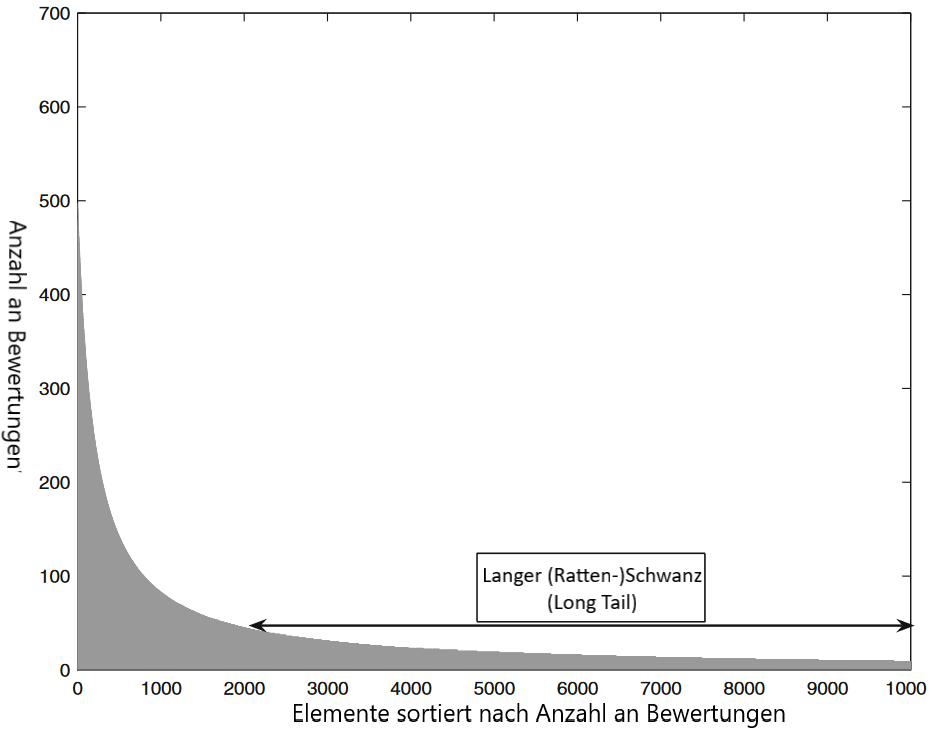
\includegraphics[width=1\textwidth]{gfx/long-tail.png}
	\caption[Darstellung des langen (Ratten-)Schwanzes]{Darstellung des langen (Ratten-)Schwanzes\\
		(Eigene Darstellung in Anlehnung an \cite[S. 33]{recommenderSystems:2016})}
	\label{fig:empfehlungssysteme:cf:speicherbasiert:abb1}
\end{figure}

Die in Abbildung \ref{fig:empfehlungssysteme:cf:speicherbasiert:abb1} dargestellte Häufigkeitsverteilung von abgegebenen Bewertungen spiegelt \textcite[S. 1ff.]{anderson:2007} zu Folge einen allgemeinen Trend wider, welchen er im Zusammenhang mit der Digitalisierung beobachtete. Der Autor stellte fest, dass sich Menschen aufgrund der heute verfügbaren breiten Angebote wesentlich diverser orientieren, als es vor einigen Jahrzehnten der Fall war \cite[S. 1ff.]{anderson:2007}.

Das Sparsity Problem kann auch in Tabelle \ref{tbl:empfehlungssysteme:arbeitsweise:tbl1} beobachtet werden. Dort haben MongoDB und Spark jeweils nur eine Bewertung. Für diese Fähigkeiten ist es über Ähnlichkeitsberechnungen im Bereich des speicherbasierten kollaborativen Filterns somit nicht möglich, für alle Angestellten robuste Vorhersagen zu ermitteln.

Um diesem Problem zu begegnen, kann die bisher verwendete Matrixdarstellung in die Form eines bipartiten Graphen überführt werden \cite[S. 2f.]{huang:2004}. Diese Datenstruktur zeichnet sich durch die Verwendung zweier unterschiedlicher Arten von Knoten zur separaten Speicherung von Nutzern und Elementen aus. Bewertungen werden bei dieser Darstellungsform über gewichtete Kanten im Graphen dargestellt \cite[S. 1f.]{cao:2021}.

Abbildung \ref{fig:empfehlungssysteme:cf:speicherbasiert:abb2} zeigt die Fähigkeitsmatrix aus Tabelle \ref{tbl:empfehlungssysteme:arbeitsweise:tbl1} in der Datenstruktur eines bipartiten Graphen. In der Darstellung sind die Knoten der Mitarbeiter rot und die Knoten der Fähigkeiten blau markiert.

\begin{figure}[h]
	\centering	
	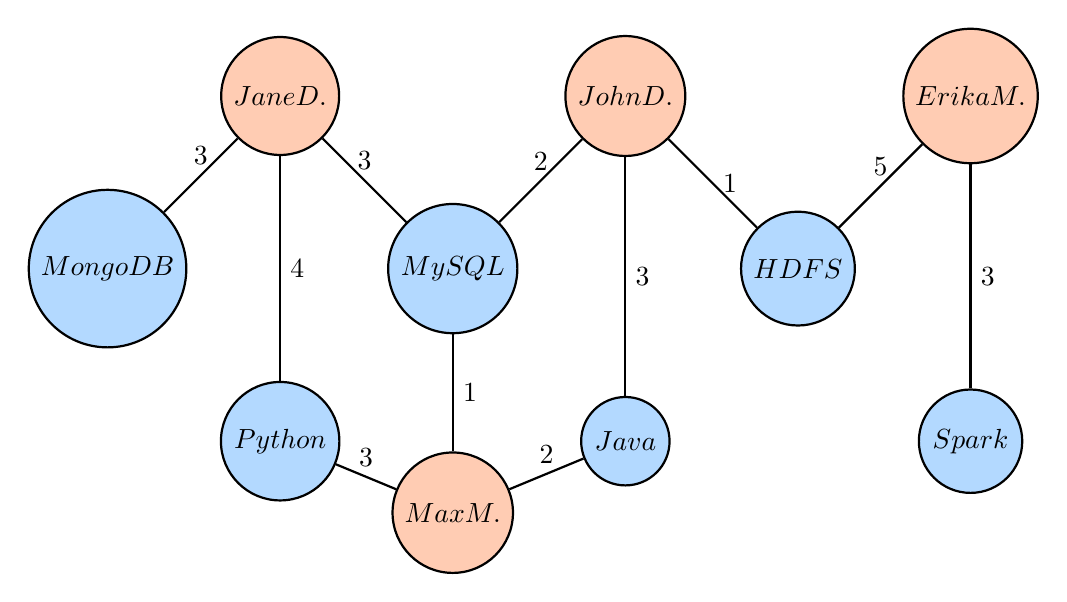
\begin{tikzpicture}[node distance={31mm}, thick, main/.style = {draw, circle}] 
		\node[main, fill=itemcolor] (MongoDB) {$MongoDB$}; 
		\node[main, fill=itemcolor] (Python) [below right of=MongoDB] {$Python$}; 
		\node[main, fill=itemcolor] (MySQL) [above right of=Python] {$MySQL$}; 
		\node[main, fill=itemcolor] (Java) [below right of=MySQL] {$Java$}; 
		\node[main, fill=itemcolor] (HDFS) [above right of=Java] {$HDFS$}; 
		\node[main, fill=itemcolor] (Spark) [below right of=HDFS] {$Spark$};
		
		\node[main, fill=usercolor] (Jane) [above right of=MongoDB] {$Jane D.$}; 
		\node[main, fill=usercolor] (John) [above left of=HDFS] {$John D.$}; 
		\node[main, fill=usercolor] (Max) [below of=MySQL] {$Max M.$};
		\node[main, fill=usercolor] (Erika) [above right of=HDFS] {$Erika M.$}; 
		
		\draw (Jane) -- node[midway, right] {4} (Python);
		\draw (Jane) -- node[midway, above] {3} (MySQL);
		\draw (Jane) -- node[midway, above] {3} (MongoDB);

		\draw (John) -- node[midway, right] {1} (HDFS);		
		\draw (John) -- node[midway, right] {3} (Java);
		\draw (John) -- node[midway, above] {2} (MySQL);
		
		%\path (Erika) edge[bend right=10] node[midway, right] {5} (HDFS); 
		\draw (Erika) -- node[midway, above] {5} (HDFS);
		\draw (Erika) -- node[midway, right] {3} (Spark);
		
		\draw (Max) -- node[midway, above] {2} (Java);
		\draw (Max) -- node[midway, above] {3} (Python);
		\draw (Max) -- node[midway, right] {1} (MySQL);
	\end{tikzpicture}

	\caption{Darstellung der Fähigkeitsmatrix aus Tabelle \ref{tbl:empfehlungssysteme:arbeitsweise:tbl1} in der Datenstruktur eines bipartiten Graphen}
	\label{fig:empfehlungssysteme:cf:speicherbasiert:abb2}
\end{figure}

\textcite[S. 7ff.]{huang:2004} bemerkten mit Blick auf bipartite Graphen, dass bei klassischen nachbarschaftsbasierten Algorithmen nur Empfehlungen für Knoten bestimmt werden können, welche von einem Zielknoten über drei Kanten zu erreichen sind. Somit können in Abbildung \ref{fig:empfehlungssysteme:cf:speicherbasiert:abb2} über solche Verfahren beispielsweise keine Bewertungsvorhersagen für Jane Doe und Spark oder Erika Muster und MongoDB bestimmt werden.

Um auch in solchen Fällen Empfehlungen zu generieren, ist der Einsatz graphenbasierter Algorithmen empfehlenswert. Diese können über transitive Verbindungen auch weiter entfernte Knoten in die Berechnung mit einbeziehen \cite[S. 60f.]{recommenderSystems:2016}.

Ein in der Literatur häufig angewendeter Graphenalgorithmus ist die Katz-Zentralität \cite[S. 6]{guns:2014}\cite[S. 1f.]{huang:2004}\cite[S. 1ff.]{zhan:2017}. Diese basiert auf einem im Jahr 1953 vorgestellten mathematischen Verfahren von \textcite[S. 1ff.]{katz:1953}, welches dieser zur Bestimmung von Anführern in sozialen Gruppen entwickelte. Heute nutzen graphenbasierte Empfehlungssysteme diesen Algorithmus beispielsweise zur Verbindungsvorhersage. Diese Problemstellung ist unter anderem im Bereich der sozialen Netzwerke verbreitet und verfolgt das Ziel, aus vorhandenen Kanten im Graphen bisher unbekannte Verbindungen vorherzusagen \cite[S. 1ff.]{libenNowell:2007}.

Der Katz-Algorithmus basiert auf folgender Gleichung \ref{frml:empfehlungssysteme:cf:speicherbasiert:formel4} \cite[S. 4]{libenNowell:2007}.
\begin{equation}
	(I - \beta * M)^{-1} - I
	\label{frml:empfehlungssysteme:cf:speicherbasiert:formel4}
\end{equation}
In Gleichung \ref{frml:empfehlungssysteme:cf:speicherbasiert:formel4} steht $\beta$ für eine Zahl im Bereich von \nullWert bis eins \cite[S. 6]{guns:2014}, welche jedoch stets kleiner als $1/\lambda$ sein muss. $\lambda$ entspricht dabei dem größten Eigenwert der Matrix M \cite[S. 6]{zhan:2017}. Je größer der Wert von $\beta$ angesetzt wird, desto stärker werden weit entfernte Beziehungen in der Berechnung gewichtet \cite[S. 6]{guns:2014}. Die Variable $I$ steht für die Einheitsmatrix. $M$ symbolisiert die Adjazenzmatrix des betrachteten Graphen \cite[S. 4]{libenNowell:2007} und gibt an, über welche Anzahl an Kanten die Knoten untereinander verbunden sind \cite[S. 6]{guns:2014}. Tabelle \ref{tbl:empfehlungssysteme:arbeitsweise:tbl2} zeigt die Adjazenzmatrix des Graphen aus Abbildung \ref{fig:empfehlungssysteme:cf:speicherbasiert:abb2}.

\begin{table}[h]
	\centering
	\begin{tabular}{c|c|c|c|c|c|c|c|c|c|c}
		& \begin{sideways}\textbf{Jane D.}\end{sideways} & \begin{sideways}\textbf{John D.}\end{sideways} & \begin{sideways}\textbf{Erika M.}\end{sideways} & \begin{sideways}\textbf{Max M.}\end{sideways} & \begin{sideways}\textbf{Java}\end{sideways} & \begin{sideways}\textbf{Python}\end{sideways} & \begin{sideways}\textbf{MySQL}\end{sideways} & \begin{sideways}\textbf{MongoDB}\end{sideways} & \begin{sideways}\textbf{HDFS}\end{sideways} & \begin{sideways}\textbf{Spark}\end{sideways} \\
		\hline
		\textbf{Jane D.}  & 0 & 0 & 0 & 0 & 0 & 4 & 3 & 3 & 0 & 0\\
		\textbf{John D.}  & 0 & 0 & 0 & 0 & 3 & 0 & 2 & 0 & 1 & 0\\
		\textbf{Erika M.} & 0 & 0 & 0 & 0 & 0 & 0 & 0 & 0 & 5 & 3\\
		\textbf{Max M.}   & 0 & 0 & 0 & 0 & 2 & 3 & 1 & 0 & 0 & 0\\
		\textbf{Java}     & 0 & 3 & 0 & 2 & 0 & 0 & 0 & 0 & 0 & 0\\
		\textbf{Python}   & 4 & 0 & 0 & 3 & 0 & 0 & 0 & 0 & 0 & 0\\
		\textbf{MySQL}    & 3 & 2 & 0 & 1 & 0 & 0 & 0 & 0 & 0 & 0\\
		\textbf{MongoDB}  & 3 & 0 & 0 & 0 & 0 & 0 & 0 & 0 & 0 & 0\\
		\textbf{HDFS}     & 0 & 1 & 5 & 0 & 0 & 0 & 0 & 0 & 0 & 0\\
		\textbf{Spark}    & 0 & 0 & 3 & 0 & 0 & 0 & 0 & 0 & 0 & 0
	\end{tabular}
	\caption{Anzahl an Verbindungen im Graphen aus Abbildung \ref{fig:empfehlungssysteme:cf:speicherbasiert:abb2}}
	\label{tbl:empfehlungssysteme:arbeitsweise:tbl2}
\end{table}

Für Tabelle \ref{tbl:empfehlungssysteme:arbeitsweise:tbl2} ergeben sich mit $\beta = 0.125$ durch Anwendung des Katz-Algorithmus die in Tabelle \ref{tbl:empfehlungssysteme:arbeitsweise:tbl3} dargestellten Werte. Die vollständige Berechnung kann in Appendix \ref{ch:nebenrechnungen:katzZentralitaet} nachvollzogen werden.

\begin{table}[h]
	\centering
	\begin{tabular}{c|c|c|c|c|c|c|c|c|c|c}
		& \begin{sideways}\textbf{Jane D.}\end{sideways} & \begin{sideways}\textbf{John D.}\end{sideways} & \begin{sideways}\textbf{Erika M.}\end{sideways} & \begin{sideways}\textbf{Max M.}\end{sideways} & \begin{sideways}\textbf{Java}\end{sideways} & \begin{sideways}\textbf{Python}\end{sideways} & \begin{sideways}\textbf{MySQL}\end{sideways} & \begin{sideways}\textbf{MongoDB}\end{sideways} & \begin{sideways}\textbf{HDFS}\end{sideways} & \begin{sideways}\textbf{Spark}\end{sideways} \\ 
		\hline
		\textbf{Jane D.}  & 1.66 & 0.47 & 0.08 & 0.87 & 0.39 & 1.66 & 1.22 & 1.00 & 0.11 & 0.03\\
		\textbf{John D.}  & 0.47 & 0.42 & 0.24 & 0.37 & 0.62 & 0.37 & 0.58 & 0.18 & 0.33 & 0.09\\
		\textbf{Erika M.} & 0.08 & 0.24 & 1.17 & 0.06 & 0.10 & 0.06 & 0.10 & 0.03 & 1.39 & 0.81\\
		\textbf{Max M.}   & 0.87 & 0.37 & 0.06 & 0.60 & 0.54 & 1.04 & 0.62 & 0.33 & 0.08 & 0.02\\
		\textbf{Java}     & 0.39 & 0.62 & 0.10 & 0.54 & 0.37 & 0.40 & 0.37 & 0.15 & 0.14 & 0.04\\
		\textbf{Python}   & 1.66 & 0.37 & 0.06 & 1.04 & 0.40 & 1.22 & 0.84 & 0.62 & 0.09 & 0.02\\
		\textbf{MySQL}    & 1.22 & 0.58 & 0.10 & 0.62 & 0.37 & 0.84 & 0.68 & 0.46 & 0.13 & 0.04\\
		\textbf{MongoDB}  & 1.00 & 0.18 & 0.03 & 0.33 & 0.15 & 0.62 & 0.46 & 0.37 & 0.04 & 0.01\\
		\textbf{HDFS}     & 0.11 & 0.33 & 1.39 & 0.08 & 0.14 & 0.09 & 0.13 & 0.04 & 0.91 & 0.52\\
		\textbf{Spark}    & 0.03 & 0.09 & 0.81 & 0.02 & 0.04 & 0.02 & 0.04 & 0.01 & 0.52 & 0.31
	\end{tabular}
	\caption{Ergebnisse des Katz-Algorithmus mit $\beta = 0.125$ für Tabelle \ref{tbl:empfehlungssysteme:arbeitsweise:tbl2}}
	\label{tbl:empfehlungssysteme:arbeitsweise:tbl3}
\end{table}

In Tabelle \ref{tbl:empfehlungssysteme:arbeitsweise:tbl3} ist zu erkennen, dass durch Berechnung des Algorithmus von Katz Verbindungen für sämtliche Knoten vorhergesagt werden konnten. Das Sparsity Problem wurde somit behoben.

Bei Betrachtung der Werte in Tabelle \ref{tbl:empfehlungssysteme:arbeitsweise:tbl3} ist festzustellen, dass das Verfahren von Katz nicht dazu geeignet ist, fehlende Mitarbeiter-Bewertungen vorherzusagen. Die Anwendung des Verfahrens führt jedoch zu einer feingranularen Anpassung der Ausgangsbewertungen auf einem veränderten Skalenniveau. So beurteilte beispielsweise Jane Doe die Kompetenzen MongoDB und \hyphenation{MySQL} in Tabelle \ref{tbl:empfehlungssysteme:arbeitsweise:tbl1} ursprünglich mit gleichen Bewertungen. Nach Berechnung des Katz-Algorithmus ist MySQL in Tabelle \ref{tbl:empfehlungssysteme:arbeitsweise:tbl3} feingranular besser bewertet als MongoDB. Dieses Phänomen ist darauf zurückzuführen, dass MySQL von mehreren Kollegen Jane Does ebenfalls bewertet wurde. Somit ist es naheliegend, dass sie diese Kompetenz besser beherrscht als MongoDB.

Nah verwandt mit dem Verfahren von Katz ist der PageRank-Algorithmus \cite[S. 1]{was:2018}. Dieser nutzt Kanten zur Darstellung von Verlinkungen im Internet. Auf dieser Grundlage bestimmte Google in seiner Anfangszeit die Priorisierung von Webseiten in deren Suchergebnissen \cite[S. 3ff.]{page:1999}.

Unabhängig von der konkreten Art der Implementierung ist ein großer Nachteil speicherbasierter Verfahren, dass bei jeder Empfehlungsberechnung sämtliche Nutzer, Elemente und Bewertungen in den Hauptspeicher geladen werden müssen \cite[S. 8]{yang:2016}. Laut \textcite[S. 3]{landherr:2010} besitzt alleine die Invertierung der Matrix bei Berechnung des Katz-Algorithmus mit Gleichung \ref{frml:empfehlungssysteme:cf:speicherbasiert:formel4} eine Komplexität von $O(n^3)$. Somit können speicherbasierte Methoden zu sehr hohen Laufzeiten führen \cite[S. 2]{zhang:2010}. Aus diesem Grund ist die Verwendung speicherbasierter Ansätze bei großen Datensätzen als ungeeignet zu bewertet. Abhilfe bei steigender Datenmenge können modellbasierte Verfahren bieten \cite[S. 8]{yang:2016}.

\subsection{Modellbasierte Verfahren}
\label{ch:empfehlungssysteme:cf:modellbasiert}
Modellbasierte Verfahren verwenden Ansätze aus dem Bereich des Data Minings zur Generierung von Vorschlägen. Hierbei berechnen Wissenschaftler statistische Modelle, bevor sie ihr Empfehlungssystem den Nutzern zur Verfügung stellen \cite[S. 2]{cui:2020}. Dieses Vorgehen hat den Vorteil, dass in der Produktivumgebung keine Berechnungen auf allen Daten ausgeführt werden müssen. Somit ist die Vorschlagsbestimmung insbesondere bei großen Datenmengen effizienter als bei speicherbasierten Verfahren \cite[S. 8]{yang:2016}.

Wie in Tabelle \ref{tbl:empfehlungssysteme:cf:modellbasiert:tbl1} dargestellt, ist es bei modellbasierten Verfahren üblich, den vorhandenen Datensatz in Trainings- (rot) und Testdaten (blau) zu untergliedern \cite[S. 71f.]{recommenderSystems:2016}. Die Einteilung in der Tabelle erfolgte zufällig.
\newpage
\begin{table}[h]
	\centering
	\begin{tabular}{c|c|c|c|c|c|c}
		& \textbf{Java} & \textbf{Python} & \textbf{MySQL} & \textbf{MongoDB} & \textbf{HDFS} & \textbf{Spark}\\ 
		\hline
		\textbf{Doe, Jane} & ? & \cellcolor{itemcolor}4 & \cellcolor{itemcolor}3 & \cellcolor{usercolor}3 & ? & ?\\
		\textbf{Doe, John} & \cellcolor{itemcolor}3 & ? & \cellcolor{usercolor}2 & ? & \cellcolor{usercolor}1 & ?\\
		\textbf{Muster, Erika} & ? & ? & ? & ? & \cellcolor{itemcolor}5 & \cellcolor{usercolor}3\\
		\textbf{Muster, Max} & \cellcolor{itemcolor}2 & \cellcolor{usercolor}3 & \cellcolor{itemcolor}1 & ? & ? & ?\\
	\end{tabular}
	\caption{Beispielhafte Unterteilung einer Matrix in Trainings- und Testdaten}
	\label{tbl:empfehlungssysteme:cf:modellbasiert:tbl1}
\end{table}

Die Trainingsdaten werden genutzt, um statistische Modelle zur Vorhersage von Bewertungen zu entwickeln \cite[S. 71f.]{recommenderSystems:2016}. Die Testdaten dienen zur anschließenden Evaluation und Bewertung hinsichtlich der Genauigkeit des erstellten Modells. Hierbei ist es beispielsweise möglich, bekannte Einträge von Testdaten in der Matrix temporär zu entfernen, diese anschließend durch das trainierte Modell vorherzusagen und daraufhin tatsächliche und vorhergesagte Werte zu vergleichen \cite[S. 3ff.]{kang:2016}.

Wie an den Spalten in Tabelle \ref{tbl:empfehlungssysteme:cf:modellbasiert:tbl1} zu erkennen ist, existieren in der Praxis häufig sehr viele Merkmale bzw. Dimensionen, welche zur Entwicklung von Modellen relevant sein können. Wie in Kapitel \ref{ch:empfehlungssysteme:cf:speicherbasiert} beschrieben, sind Matrizen in der Praxis zusätzlich aufgrund des Sparsity Problems meist sehr schwach besetzt. \textcite[S. 1]{boratto:2014} stellten fest, dass in solchen Situationen, in welchen viele Dimensionen und gleichzeitig wenige Daten vorliegen, keine statistisch aussagekräftigen Modelle erstellt werden können. \textcite[S. 94, Z. 7]{bellman:1961} prägte für diesen Sachverhalt den Ausdruck "Fluch der Dimensionalität"\footnote{"Curse of Dimensionality" - \textcite[S. 94, Z. 7]{bellman:1961}}. Um in solchen Situationen dennoch Empfehlungen generieren zu können, stellten verschiedene Autoren in der Literatur Verfahren zur Dimensionsreduzierung vor. Verbreitet ist beispielsweise die Hauptkomponentenanalyse, welche im englischsprachigen Raum als \ac{PCA} bezeichnet wird \cite[S. 1ff.]{vaswani:2018}.

\textcite[S. 1f.]{pennock:2000} kritisierten an modellbasierten Verfahren, dass diese stets den Zustand der Daten zum Zeitpunkt des Trainings des Modells abbilden. Werden beispielsweise Fähigkeiten in der Datenbank hinzugefügt bzw. entfernt oder Bewertungen signifikant verändert, muss gegebenenfalls das statistische Modell neu trainiert werden, um diese Anpassungen zu erfassen. Speicherbasierte Verfahren können den Autoren zu Folge solche Änderungen dagegen unmittelbar berücksichtigen \cite[S. 1f.]{pennock:2000}.

Ein Problem, welches weder speicher- noch modellbasierte Verfahren im Bereich des kollaborativen Filterns zuverlässig lösen können, ist der sogenannte Kaltstart. Dieser tritt auf, wenn neue Nutzer oder Fähigkeiten in die Datenbank hinzugefügt werden, welchen noch keine Bewertung zugeordnet ist \cite[S. 5]{huang:2004}. In solchen Fällen ist die gesamte Zeile bzw. Spalte in Tabelle \ref{tbl:empfehlungssysteme:arbeitsweise:tbl1} mit fehlenden Einträgen gekennzeichnet. Im entsprechenden Graphen in Abbildung \ref{fig:empfehlungssysteme:cf:speicherbasiert:abb2} existiert somit keine Kante von der betrachteten Entität zu anderen Knoten. Daher ist es weder über speicherbasierte Ähnlichkeitsberechnungen, noch graphenbasierte Algorithmen oder statistische Modelle möglich, zuverlässige Vorhersagen mittels kollaborativem Filtern zu bestimmen. Eine Lösung für die Problematik des Kaltstarts können Verfahren im Bereich des inhaltsbasierten Filterns bieten. % TODO: Quelle

\section{Inhaltsbasiertes Filtern}
\label{ch:empfehlungssysteme:inhaltsbasiertesFiltern}
Verfahren des inhaltsbasierten Filterns nutzen im Unterschied zum kollaborativen Filtern keine Bewertungen anderer Anwender zur Bestimmung von Vorhersagen. Algorithmen in diesem Bereich fokussieren Beschreibungen von Nutzern und Elementen \cite[S. 139f.]{recommenderSystems:2016}.

Soll analog zum Beispiel aus Kapitel \ref{ch:empfehlungssysteme:cf:speicherbasiert} die Java-Bewertung von Jane Doe vorhergesagt werden, würden beim inhaltsbasierten Filtern somit keine Ähnlichkeitsberechnungen zwischen Java und jeder anderen Fähigkeit bzw. Jane Doe und allen anderen Mitarbeitern durchgeführt werden. Stattdessen könnten beispielsweise Satzbausteine im Lebenslauf von Jane Doe mit Wörtern in Stellenausschreibungen für Java-Entwickler verglichen werden. Auf einem solchen Vorgehen aufbauende Anwendungen zur Stellensuche bzw. -besetzung implementierten beispielsweise \textcite[S. 4ff.]{guo:2016} und \textcite[S. 3ff.]{prospect:2010}.

Auch ist es möglich, graphenbasierte Verfahren im Bereich des inhaltsbasierten Filterns  einzusetzen. Diese bieten die Möglichkeit, vorhandene Daten über Ontologien miteinander zu verbinden. Hierbei kann auf einfache Weise zusätzliches Domänenwissen in den Vorschlagsprozess einbezogen werden. Empfehlungssysteme, welche ein solches Vorgehen verfolgen, werden als wissensbasiert bezeichnet \cite[S. 168f.]{recommenderSystems:2016}.

\section{Wissensbasierte Empfehlungssysteme}
\label{ch:empfehlungssysteme:wissensbasierteAnsaetze}
Beim Erstellen wissensbasierter Empfehlungssystemen können Unternehmen auf bereits vorhandene Ontologien zurückgreifen. Beispielsweise stellt die Europäische Kommission mit der \ac{ESCO}-Ontologie explizit zum Zweck der Stellenbesetzung eine mehrsprachige Wissensdatenbank mit vordefinierten Kompetenzen, Fähigkeiten und Qualifikationen bereit \cite[S. 1ff.]{leVrang:2014}. Ein vergleichbares Angebot existiert mit dem \ac{ONet} auch von der Regierung der Vereinigten Staaten von Amerika \cite[S. 2]{aCombinedRepresentation:2018}.

In solchen Wissensdatenbanken können Unternehmen zu Stellen passende Mitarbeiter über semantische Suchen abfragen. Hierbei kann das System über hinterlegte Regeln sowohl Synonyme als auch Beziehungen berücksichtigen \cite[S. 2f.]{singto:2013}. Jedoch werden Mitarbeiter in den Ergebnissen nur ausgegeben, wenn sie die Suchanfrage exakt erfüllen. Aus diesem Grund stellten \textcite[S. 3]{bianchini:2008} bei semantischen Suchen eine hohe Genauigkeit der Resultate fest, bemängelten jedoch die Flexibilität der Verfahren.

Auch ist es möglich, innerhalb der Ontologien über Graphenalgorithmen die Übereinstimmungen zwischen Fähigkeiten zu berechnen \cite[S. 1f.]{balachander:2018}. Bei solchen, auf Ähnlichkeitsberechnungen basierenden Verfahren beobachteten \textcite[S. 4]{bianchini:2008} eine hohe Flexibilität, kritisierten jedoch die mangelnde Genauigkeit.

Um solche Nachteile einzelner Empfehlungsansätze auszugleichen, ist es möglich, mehrere Vorschlagsverfahren innerhalb eines Systems zu kombinieren. Derartige Anwendungen werden auch als hybride Empfehlungssysteme bezeichnet \cite[S. 200]{recommenderSystems:2016}.

\section{Hybride Empfehlungssysteme}
\label{ch:empfehlungssysteme:hybrideEmpfehlungssysteme}
Durch die Verknüpfung mehrerer unterschiedlicher Empfehlungsansätze ist es mittels hybrider Systeme möglich, die Vorteile mehrerer Ansätze miteinander verbinden. Auf diese Weise kann die Qualität der Ergebnisse weiter verbessert werden \cite[S. 199f.]{recommenderSystems:2016}\cite[S. 8]{malinowski:2008}.

Beispielsweise implementierten \textcite[S. 1ff.]{combiningCbAndCFCostSensitiveApproach:2017} ein hybrides Empfehlungssystem zur Stellensuche und kombinierten dabei kollaboratives und inhaltsbasiertes Filtern über modellbasierte Methoden. Hierbei stellten sie fest, dass ihr hybrides Vorgehen zu einer höheren Präzision als der rein inhaltsbasierte Ansatz führte. \textcite[S. 1ff.]{mohamed:2018} entwickelten ein hybrides Empfehlungssystem zur Personalauswahl und kombinierten dabei wissens- und inhaltsbasierte Verfahren. Bei der Evaluation ihrer Anwendungen kamen sie zum Ergebnis, dass die Ergebnisse ihrer Anwendung vergleichbar mit der manuellen Auswahl von Personalsachbearbeitern waren. Aus diesen Resultaten schlossen sie, dass ihr hybrides Empfehlungssystem im Vergleich zu professionellen Mitarbeitern ähnlich gute Vorschläge in deutlich geringerer Zeit erzielen konnte.

Trotz solcher Ergebnisse sollte laut \textcite[S. 1ff.]{malinowski:2006} eine andere Gattung Recommender Engines zur Besetzung von Stellen implementiert werden. Den Wissenschaftlern zu Folge sollten für diese Problemstellung bilaterale Empfehlungssysteme zum Einsatz kommen. Solche Anwendungen basieren auf denen in Kapitel \ref{ch:personEnvironmentFit} vorgestellten Erkenntnissen zum \ac{PEFit} und betrachten daher gleichzeitig die Anforderungen von Personalverantwortlichen und Mitarbeitern.
\shorthandon{"}
